\documentclass[a4paper,11pt]{book}
\usepackage{listings}
\usepackage[utf8]{inputenc}
\usepackage{titlesec}
\usepackage{fancyhdr}
\usepackage[spanish,es-tabla]{babel}
\usepackage[hidelinks]{hyperref}
\usepackage{xcolor}
\usepackage{pdfpages}
\usepackage{eurosym}
\usepackage{graphicx}
\usepackage{caption}
\usepackage{subcaption}
%\usepackage{natbib}

% Información reutilizable
\newcommand{\asunto}{Trabajo de Fin de Máster}
\newcommand{\titulo}{Servicio web de GPU}
\newcommand{\tituloEng}{Web serfices of GPUs}
\newcommand{\grado}{Máster en Ingeniería Informática}
\newcommand{\autor}{José Cristóbal López Zafra}
\newcommand{\email}{tobas92@gmail.com}
\newcommand{\tutor}{Maria Isabel García Arenas}
\newcommand{\escuela}{Escuela Técnica Superior de Ingenierías Informática y de Telecomunicación}
\newcommand{\universidad}{Universidad de Granada}
\newcommand{\ciudad}{Granada}
\newcommand{\vers}{Versión 1.0}

%Comandos personalizados
\newcommand{\grad}{$^{\circ}$}

% Información archivo
\hypersetup{
	pdfauthor = {\autor\ (\email)},
	pdftitle = {\titulo},
	pdfsubject = {\asunto},
	pdfkeywords = {gpu, cuda, web service},
	pdfcreator = {LaTeX con el paquete texlive},
	pdfproducer = {pdflatex}
}



% Estilo de cabeceras
\pagestyle{fancy}
\fancyhf{}
\fancyhead[LO]{\leftmark}
\fancyhead[RE]{\rightmark}
\fancyhead[RO,LE]{\textbf{\thepage}}
\setlength{\headheight}{1.5\headheight}

% Redefinición de comandos
\renewcommand{\lstlistingname}{Fragmento de código}
\renewcommand{\lstlistlistingname}{Índice de fragmentos de código}
\renewcommand{\chaptermark}[1]{\markboth{\textbf{#1}}{}}
\renewcommand{\sectionmark}[1]{\markright{\textbf{\thesection. #1}}}

% Definición de colores
\definecolor{gray97}{gray}{.97}
\definecolor{gray75}{gray}{.75}
\definecolor{gray45}{gray}{.45}
\definecolor{gray30}{gray}{.94}
\definecolor{lightgray}{rgb}{.9,.9,.9}
\definecolor{darkgray}{rgb}{.4,.4,.4}
\definecolor{purple}{rgb}{0.65, 0.12, 0.82}
\definecolor{background}{HTML}{EEEEEE}
\definecolor{delim}{RGB}{20,105,176}
\colorlet{punct}{red!60!black}
\colorlet{numb}{magenta!60!black}

% Listados
\lstset{
	aboveskip=0.5cm,
	backgroundcolor=\color{gray97},
	basicstyle=\scriptsize\ttfamily,
	breaklines=true,
	commentstyle=\color{gray45},
	frame=Ltb,
	framerule=0.5pt,
	framesep=0pt,
	framexbottommargin=3pt,
	framexleftmargin=0.1cm,
	framextopmargin=3pt,
	keywordstyle=\bfseries,
	numberfirstline = false,
	numbers=left,
	numbersep=6pt,
	numberstyle=\tiny,
	rulesep=.4pt,
	rulesepcolor=\color{black},
	showstringspaces = false,
	stringstyle=\ttfamily,
	literate={á}{{\'a}}1
	         {é}{{\'e}}1
	         {í}{{\'i}}1
	         {ó}{{\'o}}1
	         {ú}{{\'u}}1
	         {ñ}{{\~n}}1
}

% Minimizar fragmentado de listados
\lstnewenvironment{listing}[1][]
	{\lstset{#1}\pagebreak[0]}{\pagebreak[0]}

% Listado definido para JavaScript
% http://tex.stackexchange.com/questions/89574/language-option-supported-in-listings/89576#89576
\lstdefinelanguage{javascript}{
	backgroundcolor=\color{background},
	basicstyle=\footnotesize,
	breaklines=true,
	captionpos=b,
	comment=[l]{//},
	commentstyle=\color{purple}\ttfamily,
	frame=lines,
	identifierstyle=\color{black},
	keywordstyle=\color{blue}\bfseries,
	morecomment=[s]{/*}{*/},
	morestring=[b]',
	morestring=[b]",
	ndkeywordstyle=\color{darkgray}\bfseries,
	numbers=left,
	numbersep=8pt,
	numberstyle=\scriptsize,
	sensitive=false,
	showstringspaces=false,
	stepnumber=1,
	stringstyle=\color{red}\ttfamily,
	keywords={
		break,
		case,
		catch,
		catch,
		do,
		else,
		false,
		function,
		if,
		in,
		new,
		null,
		return,
		switch,
		true,
		typeof,
		var,
		while},
	ndkeywords={
		boolean,
		class,
		export,
		implements,
		import,
		this,
		throw}
}

% Listado definido para JSON
% http://tex.stackexchange.com/questions/83085/how-to-improve-listings-display-of-json-files/83100#83100
\lstdefinelanguage{json}{
	backgroundcolor=\color{background},
	basicstyle=\footnotesize,
	breaklines=true,
	captionpos=b,
	frame=lines,
	numbers=left,
	numbersep=8pt,
	numberstyle=\scriptsize,
	showstringspaces=false,
	stepnumber=1,
	literate=
		*{:}{{{\color{punct}{:}}}}{1}
		{,}{{{\color{punct}{,}}}}{1}
	    {\{}{{{\color{delim}{\{}}}}{1}
	    {\}}{{{\color{delim}{\}}}}}{1}
	    {[}{{{\color{delim}{[}}}}{1}
	    {]}{{{\color{delim}{]}}}}{1}
	    {ñ}{{\~{n}}}{1}
}

% Para que las páginas en blanco no tengan cabecera
\makeatletter
\def\clearpage{%
  \ifvmode
    \ifnum \@dbltopnum =\m@ne
      \ifdim \pagetotal <\topskip
        \hbox{}
      \fi
    \fi
  \fi
  \newpage
  \thispagestyle{empty}
  \write\m@ne{}
  \vbox{}
  \penalty -\@Mi
}
\makeatother

\begin{document}
 \begin{titlepage}
\newlength{\centeroffset}
\setlength{\centeroffset}{-0.5\oddsidemargin}
\addtolength{\centeroffset}{0.5\evensidemargin}

\noindent\hspace*{\centeroffset}\begin{minipage}{\textwidth}

\centering

\includegraphics[width=0.9\textwidth]{../images/logo_ugr.png}\\[1.4cm]

\textsc{\Large\asunto\\[0.2cm]}
\textsc{\grado}\\[1cm]

{\Huge\bfseries \titulo\\}
\noindent\rule[-1ex]{\textwidth}{3pt}\\[3.5ex]
\end{minipage}

\vspace{2cm}
\noindent\hspace*{\centeroffset}\begin{minipage}{\textwidth}
\centering


\textbf{Autor}\\ {\autor}\\[2.5ex]
\textbf{Tutor}\\ {\tutor}\\[1cm]

\includegraphics[width=0.3\textwidth]{../images/logo_etsiit.png}\\[0.7cm]
\textsc{\escuela}\\
\textsc{---}\\
\ciudad, \today\\
\textsc{}\\[0.5cm]

\includegraphics[width=0.2\textwidth]{../images/CC-SA-logo.png}
\end{minipage}
\end{titlepage}

 \frontmatter
 \begin{center}
{\LARGE\bfseries\titulo}\\
\end{center}

\begin{center}
	Funciones de optimización en algoritmos genéticos
\end{center}

\begin{center}
	\autor\
\end{center}


\begin{figure}[h]
\centering

\includegraphics[width=0.2\linewidth]{../images/logo_swgpu}
\caption[Logo de SWGPU]{Logo de SWGPU}
\label{fig:logo}
\end{figure}

\newpage




 \begingroup
 \let\cleardoublepage\clearpage
  \tableofcontents
  \listoffigures
  %\listoftables
  %\lstlistoflistings
 \endgroup

 \newpage
 \thispagestyle{empty}
 \
 \mainmatter
\chapter{Resumen}

\section{Resumen y palabras clave}
\noindent{\textbf{Palabras clave}: \textit{servicio web}, \textit{C++}, \textit{GPU},\textit{evaluación de algoritmos}, \textit{CUDA}.\\


\bigskip
En este trabajo se aborda la creación de un conjunto de clases que permitan lanzar algoritmos genéticos y ser optimizados. Para un máximo rendimiento se paralelizarán los algoritmos, haciendo uso de una GPU.

Acceder a esas funcionalidades será posible desde un servicio web que interactue con dichas clases.


\bigskip
Para ello se implementará una infraestructura de un servicio web y la ampliaremos a un servicio web que haga uso de GPUs: dicho servicio llamará a la GPU para lanzar un algoritmo evolutivo, y usar una función de evaluación mediante el algoritmo de Ackley o Rastrigin.

Esa infraestructura que da soporte a las llamadas del servicio usará la arquitectura de cálculo CUDA.


\bigskip
Al finalizar el trabajo se obtiene un servicio web que permite lanzar algoritmos genéticos, haciendo uso de la GPU de un servidor externo mediante CUDA.





\newpage
%\begin{center}
%{\LARGE\bfseries\tituloEng}\\
%\end{center}
%\begin{center}
%\autor\
%\end{center}

\section{Extended abstract and key words}
 
 \noindent{\textbf{Key words}: \textit{web service}, \textit{C++}, \textit{GPU},\textit{ evaluation algorithms}, \textit{CUDA}.\\


\bigskip
The main objective of this project is ...

\chapter{Objetivos y motivación}


\bigskip
Un algoritmo es una serie de pasos organizados que describe el proceso que se debe seguir, para dar solución a un problema específico. A principios de la década de 1960, en 1962 John Henry Holland ideó una de las líneas más prometedoras de la inteligencia artificial, la de los algoritmos genéticos, y con su libro ``Adaptation in Natural and Artifical Systems`` en 1975 logró una mayor popularidad. 

Son llamados así porque se inspiran en la evolución biológica y su base genético-molecular. Estos algoritmos hacen evolucionar una población de individuos sometiéndola a acciones aleatorias semejantes a las que actúan en la evolución biológica (mutaciones y recombinaciones genéticas), así como también a una selección de acuerdo con algún criterio, en función del cual se decide cuáles son los individuos más adaptados, que sobreviven, y cuáles los menos aptos, que son descartados.

\bigskip
Para su funcionamiento (el de un algoritmo genético simple, llamado Canónico), al empezar necesita una codificación o representación del problema que se adecue al mismo y una función de ajuste o adaptación al problema. Durante la ejecución del algoritmo, los padres deben ser seleccionados para la reproducción, a continuación dichos padres seleccionados se cruzarán generando dos hijos, sobre cada uno de los cuales actuará un operador de mutación. El resultado de la combinación de las anteriores funciones será un conjunto de individuos (posibles soluciones al problema), los cuales en la evolución del algoritmo genético formarán parte de la siguiente población.

\bigskip
Poseen multitud de aplicaciones, como pueden ser:

\begin{itemize}
	\item Diseño automatizado para la investigación de diseño de materiales, equipamiento industrial o sistemas de comercio en el sector financiero.
	\item Construcción de árboles filogenéticos.
	\item Diseño de sistemas de distribución de aguas.
	\item Resolución de equilibrios en Teoría de juegos.
	\item Análisis de expresión de genes.
\end{itemize}

\bigskip
Pueden resolver problemas de alta complejidad, pero esto suele traducirse en operaciones muy costosas en términos de tiempo y recursos. En la actualidad, por ejemplo, hay casos en los que recrear una simulación de la solución propuesta por una iteración puede durar varios días y consumir gran cantidad de procesamiento y recursos asociados.





\bigskip
\section{Objetivos}
\bigskip


\begin{itemize}
	
	\item Se desarrollarán varias clases para lanzar algoritmos genéticos que aprovechen el cálculo paralelo de alguna arquitectura de cálculo especializada (más adelante se vera que se opta por CUDA)
	
	\item Además se desarrollará un servicio web que interactúe con ellas. Esa infraestructura que da soporte a las llamadas del servicio debe hacer uso de una GPU. Esto hará que dichos algoritmos genéticos sean más accesibles y fáciles de usar, ya que sólo tendrán que introducir los parámetros que se deseen y lanzar el algoritmo de manera intuitiva y sin necesidad de una preparación previa.
	
	\item Y se estudiará la posibilidad de publicar dicho servicio para que sea accesible por cualquier usuario de Internet.
	
\end{itemize}



\bigskip
\section{Motivación}
\bigskip

Dicha complejidad en la resolución de los algoritmos genéticos lleva a optimizarlos y a trabajar con ellos para lograr reducir el coste de dichas operaciones. 

Esto lleva a utilizar una computación paralela, en la que se aprovecha la potencia de computación de los sistemas con los que trabajamos realizando cálculos simultáneamente. Sigue el principio de dividir los problemas grandes en problemas más pequeños, que se solucionan en paralelo para luego obtener la solución del problema inicial.

Por otra parte, en el ámbito de la computación se ha visto una gran evolución de las tarjetas gráficas, ya que grandes fabricantes como NVIDIA, AMD, IBM o Intel han logrado una producción de GPUs de gran alcance, como se puede ver en la Figura \ref{fig:gpu_vs_cpu} (pueden incluso superar la frecuencia de reloj de una CPU antigua).

\bigskip
\begin{figure}[h]
	\centering
	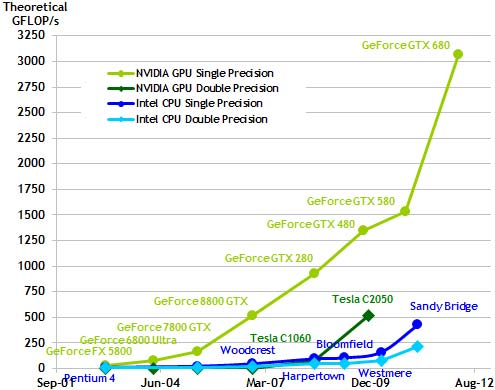
\includegraphics[width=0.7\linewidth]{../images/gpu_vs_cpu}
	\caption[Evolución de las GPUs respecto a las CPUs]{Evolución hasta 2012 de las GPUs respecto a las CPUs}
	\label{fig:gpu_vs_cpu}
\end{figure}


\bigskip
El uso de computación paralela, junto la potencia y la posibilidad de usar el paralelismo que ofrecen las GPU  hace muy interesante el uso de dichas GPUs para resolver algoritmos genéticos de formas más eficiente.

Después del estudio realizado en el siguiente capítulo, se opta por usar la arquitectura de cálculo CUDA \cite{nvidiacuda} para crear algoritmos genéticos que se ejecuten en GPUs de NVIDIA \cite{nvidiadeveloper}.

Como se cita en uno de los objetivos, se publicará de manera que cualquier usuario tenga acceso. Esto, junto a una interfaz sencilla, permitirá computar algoritmos genéticos con facilidad y rapidez.





\chapter{Estudio del arte}
\bigskip

Los principios básicos de los algoritmos genéticos fueron establecidos por Holland (1975), y se encuentran bien descritos en varios textos a lo largo de los años, como los estudios de Goldberg (1989), Davis (1991), Michalewicz (1992) o Reeves (1993), afianzando los conceptos y permitiendo trabajar sobre una buena base a futuros investigadores.

\bigskip
Son muchos y muy variados los ámbitos en los que se usan los algoritmos genéticos. Sirven para crear componentes automovilísticos, analizar expresiones de genes o hasta desarrollar aprendizajes de comportamiento para robots.

\bigskip
El poder de los algoritmos genéticos proviene del hecho de que se trata de una técnica robusta y tratan con éxito una gran variedad de problemas provenientes de diferentes ámbitos, incluyendo aquellos en los que otros métodos encuentran dificultades. Si bien no se garantiza que el algoritmo genético encuentre la solución óptima del problema, existe evidencia empírica de que se encuentran soluciones de un nivel aceptable, en un tiempo competitivo con el resto de los algoritmos de optimización combinatoria. En el caso de que existan técnicas especializadas para resolver un determinado problema, lo más probable es que se superen al Algoritmo genético, tanto en rapidez como eficacia. El gran campo de aplicación de los algoritmos genéticos se relaciona con aquellos problemas para los cuales no existen técnicas especializadas. Incluso en el caso en que dichas técnicas existan, y funcionen bien, pueden efectuarse mejoras de las mismas conjuntándolas con los algoritmos genéticos.

Esto hace que se estudie y se intente mejorar y optimizar dichos algoritmos, siendo un campo con mucha transcendencia en la actualidad.

\bigskip
Constan de varias partes, como la selección de candidatos, operadores de cruce, funciones de evaluación y optimización o mutación. En este trabajo nos centraremos en la parte de optimización, donde se evalúan los individuos generados y que serán posibles soluciones al problema.

Existen multitud de funciones de optimización, pero nos centraremos en 2: Ackley y Rastrigin.

\bigskip
La función de Ackley se publicó por primera vez en "A connectionist machine for genetic hillclimbing" por David H. Ackley en 1987 y se extendió a la dimensión arbitraria en "Evolutionary algorithms in theory and practice: evolution strategies, evolutionary programming, genetic algorithms" por Thomas Bäck en 1996.

\bigskip
\begin{figure}[h]
	\centering
	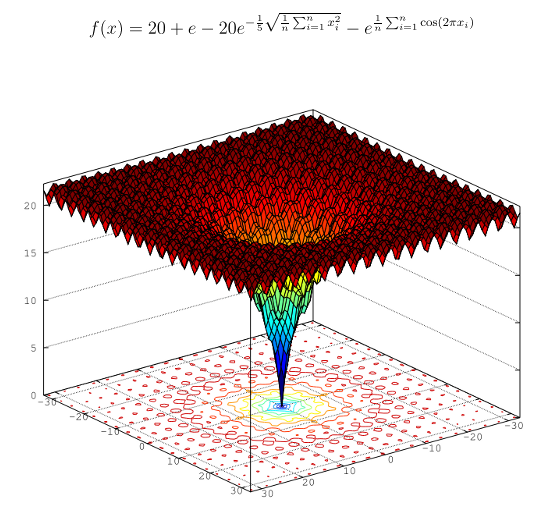
\includegraphics[width=0.7\linewidth]{../images/ackley}
	\caption[Función y representación de la función de optimización de Ackley]{Función y representación de la función de optimización de Ackley}
	\label{fig:ackley}
\end{figure}


\bigskip
Años antes, en 1974, Rastringin en "Systems of extremal control." propone otra función de optimización, para ser generalizada en 1991 por Mühlenbein.


\bigskip
\begin{figure}[h]
	\centering
	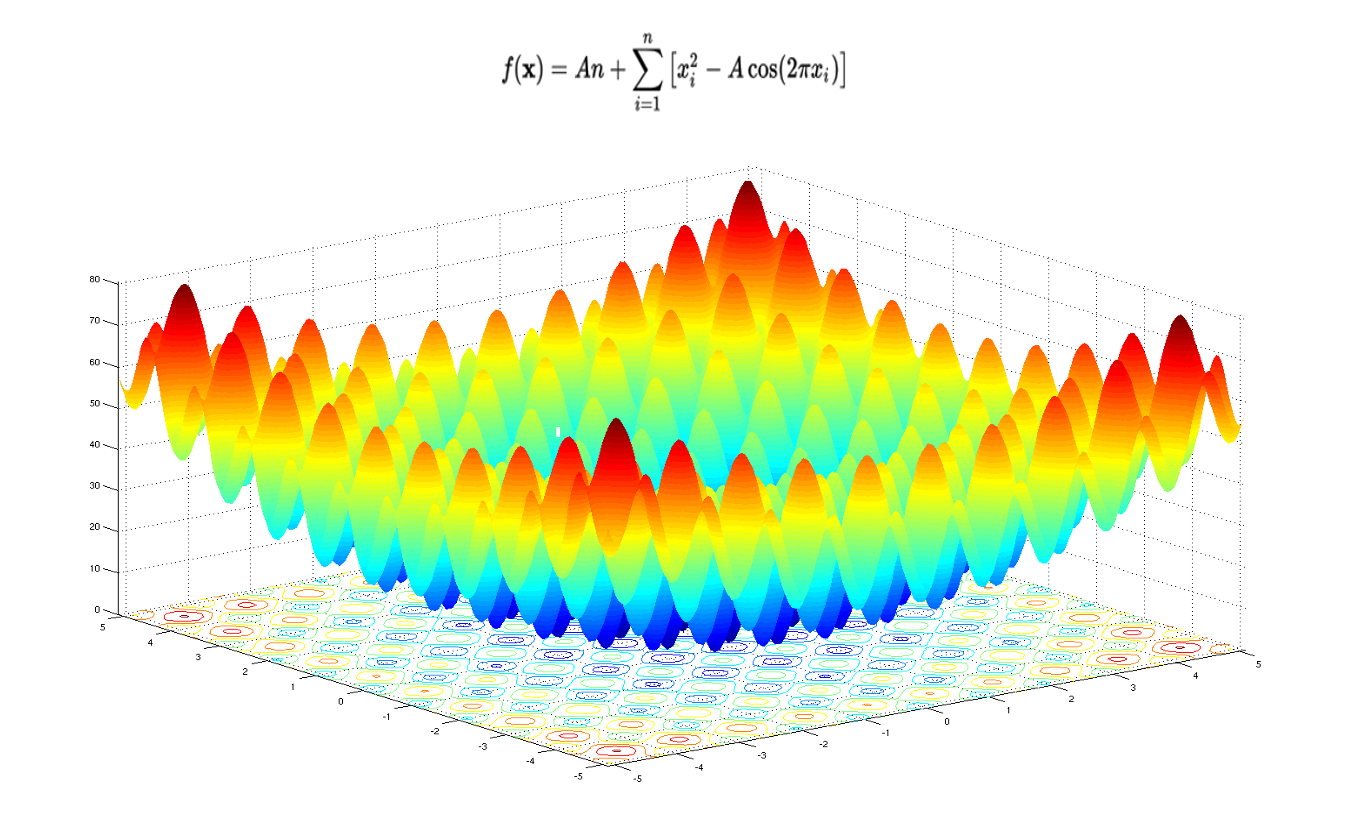
\includegraphics[width=0.7\linewidth]{../images/rastrigin}
	\caption[Función y representación de la función de optimización de Rastrigin]{Función y representación de la función de optimización de Rastrigin}
	\label{fig:rastrigin}
\end{figure}

\bigskip
En este trabajo nos centraremos en estas 2 funciones de optimización, ofreciendo un algoritmo genético que pueda ser optimizado mediante Ackley o Rastrigin.


\newpage
\section{Actualidad}
\bigskip

En la actualidad la mayoría de los usuarios que necesitan procesar un algoritmo genético lo hacen ellos mismos, con programas adaptados de terceros o desarrollados por ellos mismos. Esto conlleva un trabajo extra de estudio, implementación y corrección de dichos programas. 

Podemos encontrar algunos programas \cite{agpython} \cite{agjava} \cite{agmatlab} para ser ejecutados por el cliente, o servicios web que realizan algoritmos genéticos donde la mayoría son ejemplos o demostraciones de algoritmos genéticos y sus soluciones \cite{agandar} \cite{agcoche}.


Pero ninguno usa la computación paralela aprovechando la potencia de las GPUs. Viendo que hay disponible en el ámbito de dicha paralelización vemos que hay grandes empresas que han lanzado lenguajes de programación enfocados a aprovechar el procesamiento mediante la GPU: CUDA \cite{nvidiacuda}, AMD OpenCL APP \cite{paralelizacionamd}, BrookGPU \cite{brookgpu}, PeakStream o RapidMind:

\begin{itemize}
	\item CUDA: arquitectura de cálculo paralelo de NVIDIA. Se basa en el lenguaje C y C++, por lo que, junto con la cantidad de dispositivos de la marca, existe una gran comunidad y documentación.
	
	\item AMD OpenCL™ Accelerated Parallel Processing: herramienta de AMD que permite el cómputo mediante GPUs. Se basa en los lenguajes OpenCL y C++, por lo que se pueden usar para acelarar aplicaciones.
	
	\item BrookGPU: programa (en versión \textit{beta}) de la Universidad de Stanford para aprovechar la paralelización en tarjetas gráficas AMD y NVIDIA. Para trabajar con el se usa una extensión de ANSI C.
	
	\item PeakStream era un programa para paralelizar el procesamiento con grandes rendimientos en tarjetas AMD, comprado por Google en 2007 \cite{peackstream}, y tras esto, a dejado de ofrecer mantenimiento.
	
	\item RapidMind, que tambíen se basa en C++, es comprada por Intel en 2009 y pasa a ser Intel Array Building Blocks \cite{rapidmind}, pero sigue estando en forma experimental. 
	
\end{itemize}

Tras ver las distintas opciones, con sus distintas ventajas e inconvenientes, decidimos centrarnos en CUDA. Vemos que es un proyecto activo, tiene numerosas actualizaciones, cuenta con mucha comunidad para resolver dudas y fomentar su desarrollo, y tiene numerosas facilidades, como un SDK \cite{nvidiadeveloper} y varias herramientas para sus desarrolladores. Por todo esto escogemos CUDA para desarrollar nuestro trabajo.

En este campo hay algunos proveedores, como Impact  \cite{cudaimpact} o gpuOcelot \cite{cudagpuocelot} que ofrecen herramientas para la computación de algoritmos estándar o del código que genere el usuario, pero  realizando el cómputo desde las GPUs de los clientes, y nunca enfocados específicamente a resolver algoritmos genéticos.

Otras opciones nos permiten ejecutar CUDA en servidores externos, pero se necesita enviar una solicitud de uso y adaptarse a sus restricciones y capacidad, como en rCUDA \cite{rcuda}
o desplegar toda una instancia en un IaaS y desarrollar dentro: Amazon Web Services \cite{amazoncuda}.


Con esto vemos que podemos encontrar servicios que realicen algoritmos genéticos, o servicios que usen CUDA, pero no hay servicios que combinen ambos.


\bigskip
\section{Clientes}
\bigskip

¿Que usuarios necesitan computar algoritmos genéticos?
Por ejemplo, cualquier estudiante que quiera comprobar los cambios en los distintos parámetros del algoritmo genético.

¿Y además algoritmos que requieran mucha capacidad de cómputo? En principio el personal de investigación cumple con estas características. Junto con la potencia de cómputo y la accesibilidad que proporcionaremos simplificaríamos el trabajo de dicho personal. 

Además el servicio será accesible a cualquier usuario, y con su interfaz sencilla e intuitiva dichos usuarios no necesitarán una preparación especial para usarlo. 

\bigskip
\section{Competidores}
\bigskip

Como se cita antes, existen ejemplos o plantillas de algoritmos genéticos \cite{agpython} \cite{agjava} \cite{agmatlab} que los usuarios pueden usar, pero necesitan para su uso un trabajo extra para su instalación, desarrollo o ajustes. Además de este trabajo extra, se ven limitados por las capacidades de sus dispositivos, pues los algoritmos se tendrán que lanzar en local.

Para evitar dichas limitaciones, podemos usar la parelelización de los algoritmos, pero los trabajos que encontramos se encuentran en una versión de CUDA obsoleta \cite{paralelizacioncuda} (y simplemente exponiendo el código) o son estudios del servicio sin llegar a ser implementado \cite{optimizacionparalelizacioncuda}. Se busca entonces un servicio que ofrezca computación desde un servidor externo. Podemos ver servicios que computan directamente CUDA \cite{rcuda} u ofrecen instancias con acceso a GPUs \cite{amazoncuda}  pero nunca especializados en algoritmos genéticos.


\bigskip
\section{Conclusiones}
\bigskip

Si buscamos un servicio de computación externo (que ofrezca una mayor potencia de computación usando GPUs) de algoritmos genéticos no llegamos a encontrar nada que cumpla con nuestro requisitos: o son servicios en local para lanzar algoritmos genéticos o son servicios externos que nos ofrecen computación aprovechando la paralelización de CUDA, pero sin llegar a ofrecer ninguna aproximación de un algoritmo genético.

Viendo esto llegamos a una demanda que podemos cubrir con nuestro servicio, motivando a su desarrollo, implementación y creación.








\chapter{Requisitos}

\bigskip
Detallaremos las restricciones que se han tenido al empezar el desarrollo, los requisitos funcionales identificados, y los casos de uso.

\newpage
\section{Restricciones}


\section{Requisitos funcionales}


\section{Casos de uso}







\chapter{Tecnologías}

\bigskip
Enumeraremos y describiremos las herramientas y tecnologías de desarrollo que se han usado.

\newpage
\section{Herramientas}




\subsection{Tecnologías}








\chapter{Desarrollo del sistema}

\bigskip
En este capítulo veremos la arquitectura del sistema, la \textit{filosofía} o principios seguidos y algunas partes del sistema.

\bigskip
El código del sistema se encuentra en GitHub. Para el sistema completo, que recoge el servicio web y la gestión de la ejecución del algoritmo genético: \textcolor{blue}{\href{https://github.com/JCristobal/SWGPU}{SWGPU}}. Y para el módulo que gestiona el algoritmo genético: \textcolor{blue}{\href{https://github.com/JCristobal/geneticAlgorithm}{geneticAlgorithm}}.

\bigskip
Y se encuentra disponible, en forma de \textit{beta} en  \textcolor{blue}{\href{http://www.genmagic.ugr.es:8000}{www.genmagic.ugr.es:8000}}, accesible dentro de la red de la UGR \cite{vpnugr}.

\bigskip
\section{Arquitectura del sistema}
\bigskip

La arquitectura del sistema está compuesta por 2 capas: BackEnd y FrontEnd. La capa de BackEnd se sitúa en el servidor, mientras que la de FrontEnd en el lado del cliente.

\bigskip
La estructura básica de la web la formará desde el lado BackEnd (en el servidor) mediante Django (usando python) y será servida por el servidor Apache. 

El cliente, desde el FrontEnd, verá la web mediante HTML5, CSS3 y JavaScript, y podrá interactuar con ella fácilmente gracias a las funcionalidades de jQuery y AngularJS

Otra vez en el BackEnd, tras la petición del cliente, el algoritmo genético se ejecutará en C++ y CUDA. La respuesta se le enviará en formato JSON, para ser maquetada de forma correspondiente.


\bigskip
En la siguiente imagen (Figura \ref{fig:estructura}) se muestra con sus distintos elementos:

\bigskip
\begin{figure}[h]
	\centering
	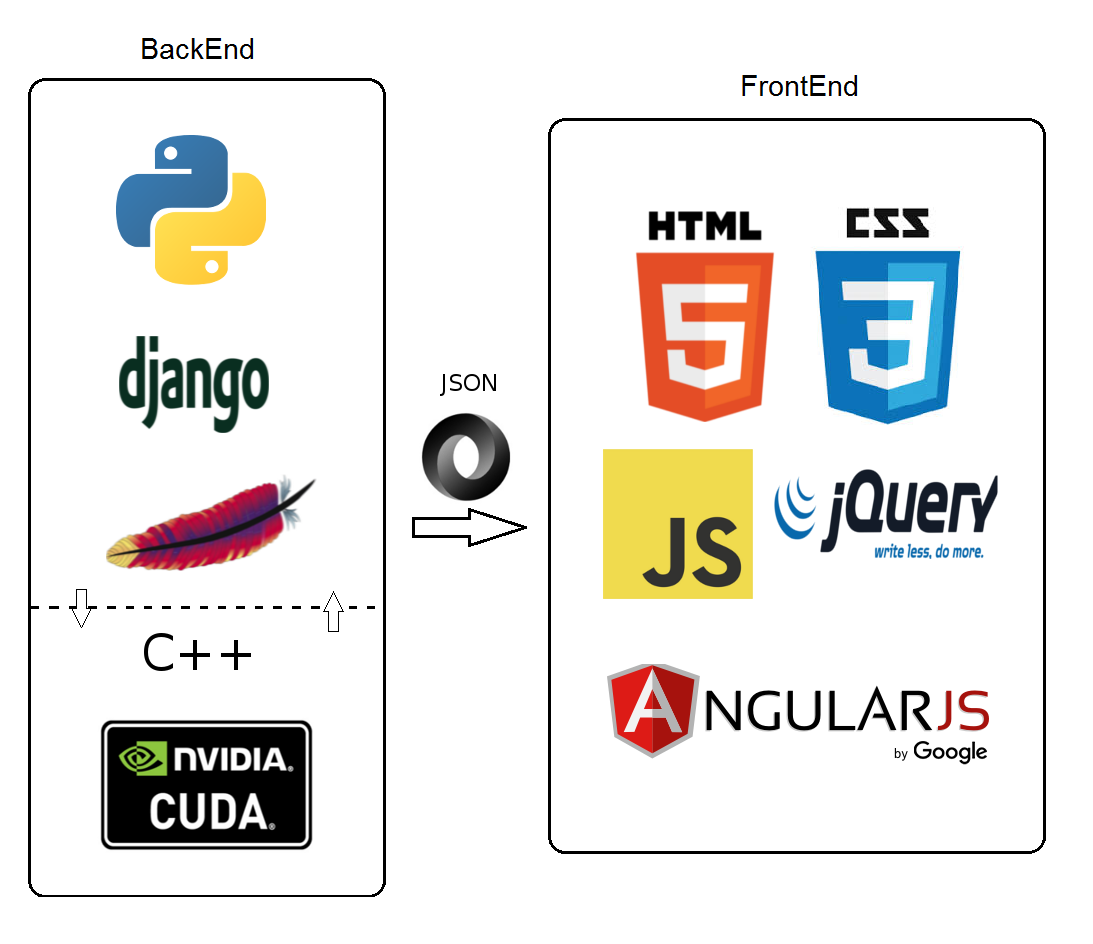
\includegraphics[width=1\linewidth]{../images/estructura}
	\caption[Estructura del sistema]{Estructura del sistema}
	\label{fig:estructura}
\end{figure}



\newpage
\section{Partes del sistema}

\bigskip
\textbf{BackEnd}\\

Será el lado del servidor de la aplicación. Basado en Django (y disponible mediante el servidor Apache), con éste tenemos acceso a los recursos del servidor, entre ellos la GPU. Con Django formaremos la petición según los parámetros que ha especificado el cliente, y se hará uso de la GPU mediante CUDA. Django tendrá la salida del cálculo, y la devolverá en un formato determinado.

Se puede decir que el BackEnd tiene 2 partes: el servidor web y el procesado dentro del servidor.

\bigskip
\textbf{FrontEnd}\\

Lado que ve el cliente, el FrontEnd. Con las tecnologías básicas web (HTML5, CSS y JavaScript) se creará una interfaz para el cliente. Mediante jQuery y AngularJS podrá interactuar fácilmente y con fluidez, además de servir la respuesta que le da el servidor.

\bigskip
AngularJS se encarga de la comunicación con el BackEnd a través de servicios, y con esos datos actualiza la interfaz. Conforma un modelo MVC (Modelo Vista Controlador), que separa los datos y su gestión (componente de modelo) de la aplicación de la interfaz de usuario (vista) y el módulo encargado de gestionar los eventos y las comunicaciones (controlador).

MVC propone la construcción de tres componentes distintos (modelo, vista y controlador): por un lado define componentes para la representación de la información, y por otro lado para la interacción del usuario. 

\bigskip
\begin{figure}[h]
	\centering
	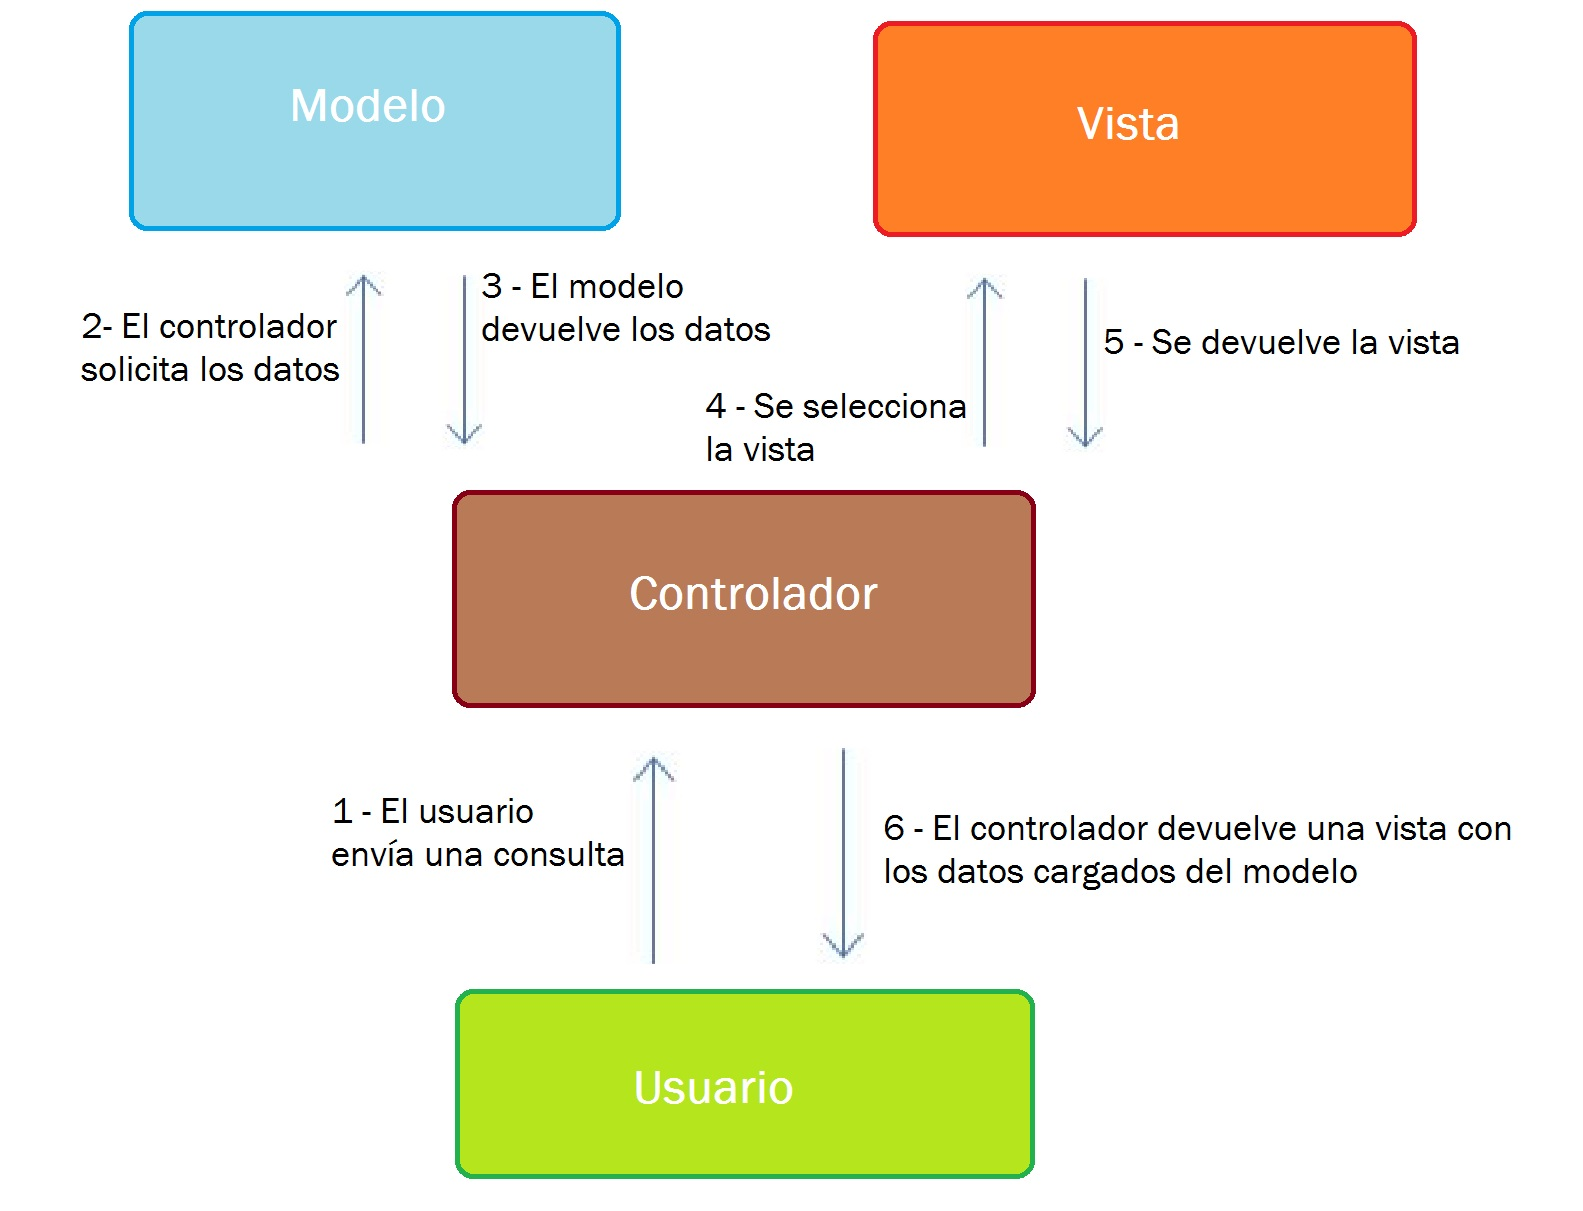
\includegraphics[width=0.8\linewidth]{../images/mvc}
	\caption[Modelo Vista Controlador]{Modelo Vista Controlador}
	\label{fig:mvc}
\end{figure}



\newpage
\section{Filosofía a seguir}
\bigskip
A la hora de implementar y de realizar el trabajo en general se ha intentado ser lo más ordenado y pulcro posible, esto en un principio  puede ralentizar el proceso, pero a largo plazo hace que el desarrollo, actualización o mantenimiento del sistema sea más rápido y fácil. Estos son algunos de los criterios empleados en el desarrollo.

\bigskip
\subsection{Desarrollo general}
\bigskip

Las funciones del sistema se han desarrollado de la manera más general posible para así favorecer la reutilización de código y facilitar su legibilidad. También son más fáciles de mantener puesto que al ser de ámbito más general son más mantenibles.

\bigskip
\subsection{Modularización}
\bigskip

Se ha desarrollado el código en distintos módulos. De esta forma se evita que al hacer cambios en un módulo se propague a los demás, lo que hace el código más mantenible y eficiente.

\bigskip
\subsection{Control de versiones}
\bigskip

Se apostó por un sistema de control de versiones, en mi caso Git mediante la plataforma GitHub \cite{github}, ya que favorece el mantenimiento de las distintas versiones de código de una manera sencilla y rápida.

El manejo de Git es sencillo, ya que con unas cuantas ordenes se puede manejar sin problemas, y GitHub está provisto de una interfaz muy intuitiva. 

\bigskip
Algunas de las órdenes que se han usado para el trabajo son:\\


\textit{git clone[URL del proyecto]}: se descarga el proyecto del repositorio Git.\\


\textit{git add [archivos]}: añade los archivos con los cambios deseados en un "paquete" para el commit.\\


\textit{git commit}: subida de los archivos especificados al repositorio local.\\


\textit{git push}: propaga los cambios locales al repositorio.\\


\textit{git pull origin}: Actualiza la versión del código.\\


\textit{git status}: muestra el estado de los archivos.\\


\bigskip
\subsection{Desarrollo iterativo incremental}
\bigskip

El desarrollo de las funcionalidades se hace de forma progresiva, de modo que primero se implementan las más críticas y prioritarias en primer lugar para poder tener siempre un producto funcional.

\bigskip
\subsection{Revisiones periódicas del código}
\bigskip

El código es revisado tras cada interacción de desarrollo, con el fin de mantenerlo lo más pulcro y estructurado posible. De este modo se evitan repeticiones en el código o dejar partes incompletas. Así se proporciona un mayor nivel de calidad a código producido.

\bigskip
\subsection{Documentación del código}
\bigskip

El código ha sido documentado, de modo que es más mantenible por terceros y por el mismo autor. Cada funcionalidad ha sido detallada debidamente, de manera clara y concisa, sin extender demasiado la explicación.




\newpage
\section{Estructura}

\bigskip
\subsection{FrontEnd}
\bigskip

Sigue el modelo que recomienda AngularJS, como antes se cita, se basa en el modelo MVC. Los distintos tipos de archivos que formarán las \textit{vistas} (en distintas ubicaciones según la forma de Django) son:

\begin{itemize}
	\item HTML (dentro del directorio \textit{templates}) será la plantilla visible del sistema.
	\item CSS: (en el directorio \textit{static/assets/css}) estilos que usará HTML.
	\item JavaScript (dentro de \textit{static/assets/js}) mediante jQuery y AngularJS permitirán interactuar con el sistema.
	\item Las imágenes y distintas librerías que se usen también se ubicarán en \textit{static/assets}.
\end{itemize}


\bigskip
\subsection{BackEnd}
\bigskip

Se hará uso de Django para crearlo y gestionarlo. A continuación se citan sus partes importantes que se usan en el proyecto:

\begin{itemize}

	\item \textbf{manage.py}: archivo para gestionar el proyecto (inspeccionarlo en busca de problemas, lanzar el servidor o cargar datos).
	\item \textbf{settings.py}: configuraciones del proyecto (dirección de algunos directorios o carga de módulos con distintas funcionalidades)
	
	Dentro del directorio \textit{swgpu} (que será un \textit{packete python}):
	\begin{itemize}
		\item \textbf{urls.py}: URL declaradas dentro del proyecto \textit{swgpu}.
		\item \textbf{views.py}: para gestionar las vistas y las funcionalidades del proyecto.
	\end{itemize}
	
	
	\item La parte de FrotEnd antes descrita se situará en los directorios \textit{templates} y \textit{static}. Django hará uso de los distintos archivos dentro para lanzar y trabajar con el servicio web.
\end{itemize}

\bigskip
\subsection{Ejecutable a usar por el BackEnd}
\bigskip

El sistema hará uso de la GPU del servidor (BackEnd) mediante el ejecutable \textit{geneticAlgorithm} (ubicado en el directorio \textit{bin}), escrito en C++ y CUDA. De esta manera se facilitará el servicio, ya que al tratarse de un ejecutable al que sólo hay que realizar una petición con los parámetros deseados se cubren los posibles fallos y la salida que dará. 

\bigskip
En las siguiente imagen se ve una captura de petición de ayuda sobre las variables a introducir mediante el ejecutable:

\bigskip
\begin{figure}[h]
	\centering
	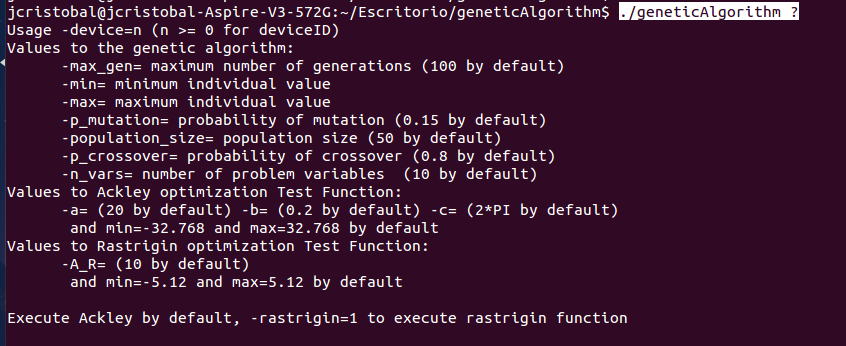
\includegraphics[width=1\linewidth]{../images/peticion_ejecutable}
	\caption[Petición de un algoritmo genético mediante el ejecutable]{Petición de un algoritmo genético mediante el ejecutable}
	\label{fig:peticion_ejecutable}
\end{figure}

\bigskip
Y otra captura con una petición que ejecutaría el algoritmo genético con los parámetros especificados además de los declarados por defecto:

\bigskip
\begin{figure}[h]
	\centering
	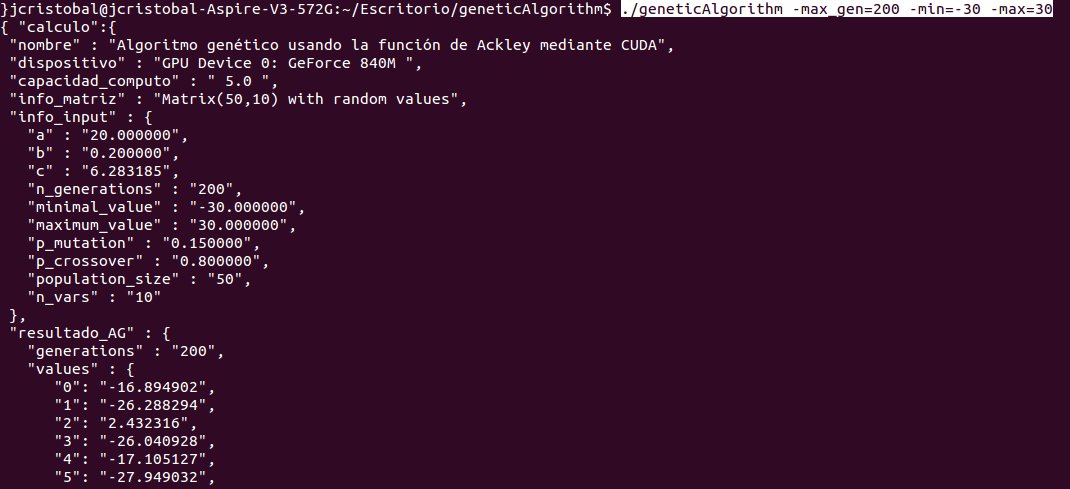
\includegraphics[width=1\linewidth]{../images/salida_ejecutable}
	\caption[Salida del algoritmo genético]{Salida del algoritmo genético}
	\label{fig:salida_ejecutable}
\end{figure}

\bigskip
y a continuación se ve la salida completa en formato JSON:

\begin{lstlisting}
{
	"calculo": {
		"nombre": "Algoritmo genético usando la función de Ackley mediante CUDA",
		"dispositivo": "GPU Device 0: GeForce 840M ",
		"capacidad_computo": " 5.0 ",
		"info_input": {
			"a": "20.000000",
			"b": "0.200000",
			"c": "6.283185",
			"n_generations": "200",
			"minimal_value": "-30.0000",
			"maximum_value": "30.0000",
			"p_mutation": "0.150000",
			"p_crossover": "0.800000",
			"population_size": "50",
			"n_vars": "10"
		},
		"resultado_AG": {
			"generations": "200",
			"values": {
				"0": "-16.894902",
				"1": "-26.288294",
				"2": "2.432316",
				"3": "-26.040928",
				"4": "-17.105127",
				"5": "-27.949032",
				"6": "25.647144",
				"7": "-7.420090",
				"8": "-0.034110",
				"9": "13.586363"
			},
			"best_fitness": "0.000000"
		},
		"datos_computo": {
			"performance": "9846.59 Flop/s",
			"time": "50.779 msec",
			"size": "500 ps",
			"workgroupSize": "50 threads/block"
		}
	}
}
\end{lstlisting}


\bigskip
Se optó por un ejecutable porque si cada vez que se realizara una petición hubiese que compilar el programa con el algoritmo genético, comprobar que no hubiese fallos ni generase errores, y no se garantizaría una salida formateada correctamente, además de generar una petición que consume más recursos y tiempo.

\bigskip
Pese a todas esas desventajas, se podría permitir al usuario cambiar el código fuente, o añadir funcionalidades y con un buen uso por su parte y una correcta prevención de fallos se conseguiría una funcionalidad mayor y llena de posibilidades. Pero como esta posibilidad no se ofrece en este trabajo, se hablará en el capítulo 8 sobre ella.


\newpage
\section{Pruebas}
\bigskip

A continuación se probará el rendimiento en 2 dispositivos distintos con sus respectivas especificaciones para realizar el cómputo. Con esto se verá que el sistema no depende de un modelo específico de tarjeta y presenta buenos resultados para varios modelos.

Se probará para una tarjeta GeForce 840M \cite{geforce840m} y GeForce GXT 660 Ti \cite{geforcegtx660}. Primero se verá una comparativa entre ambas, para luego ver los resultados obtenidos al realizar los mismo cómputos.

\bigskip
\begin{figure}[h]
	\centering
	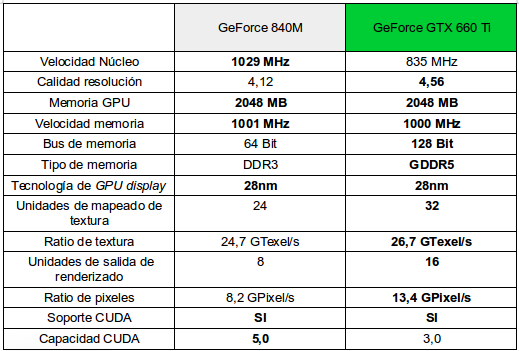
\includegraphics[width=1\linewidth]{../images/especificaciones}
	\caption[Especificaciones de las tarjetas 840M y GTX660]{Especificaciones de las tarjetas 840M y GTX660}
	\label{fig:especificaciones}
\end{figure}

\bigskip
Como nota hay que destacar el parámetro de \textit{capability} (capacidad), que será el que mayores restricciones o mejoras imponga en sus distintas versiones. Cuanto mayor sea esta, más funcionalidades podrá realizar y soportará más requisitos técnicos.

\bigskip
En la siguiente gráfica (Figura \ref{fig:grafico_benchmarks}) se verá la diferencia de ambas en benchmarks para medir \underline{procesamiento de gráficos} (Parallax, MRender, Gravity y Splatting):

\begin{figure}[h]
	\centering
	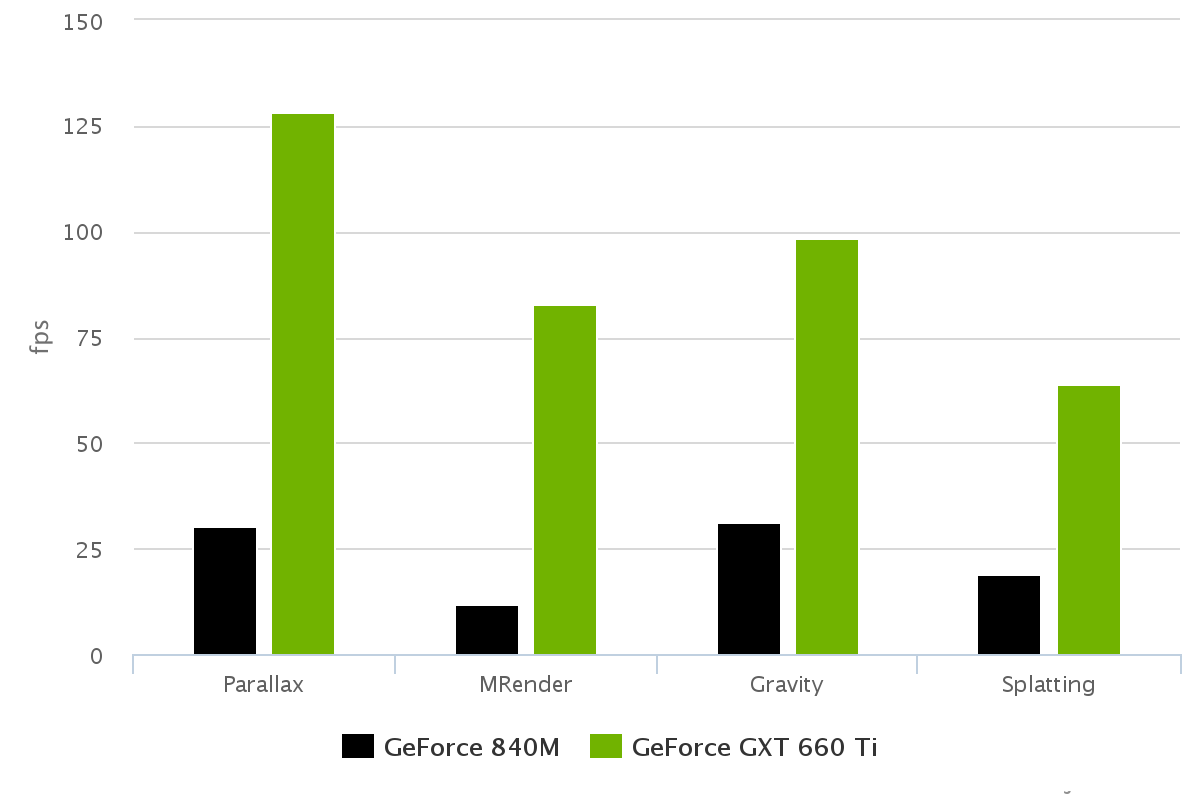
\includegraphics[width=0.6\linewidth]{../images/grafico_benchmarks}
	\caption[Comparativa de las tarjetas mediante bencharks de GPU]{Comparativa de las tarjetas mediante bencharks de GPU}
	\label{fig:grafico_benchmarks}
\end{figure}


\newpage %\bigskip
Pero en el ámbito de la computación mediante GPU con CUDA tendremos hay que fijarse en la capacidad de cada modelo de tarjeta, ya que una versión más actualizada puede lograr mejores resultados aunque tenga peores especificaciones \cite{capacidadescuda}.

\bigskip
Para ello se verán los tiempos que emplean ambas tarjetas (con distintas capacidades \cite{capacidades}) para varios números de generaciones:

\bigskip
\begin{figure}[h]
	\centering
	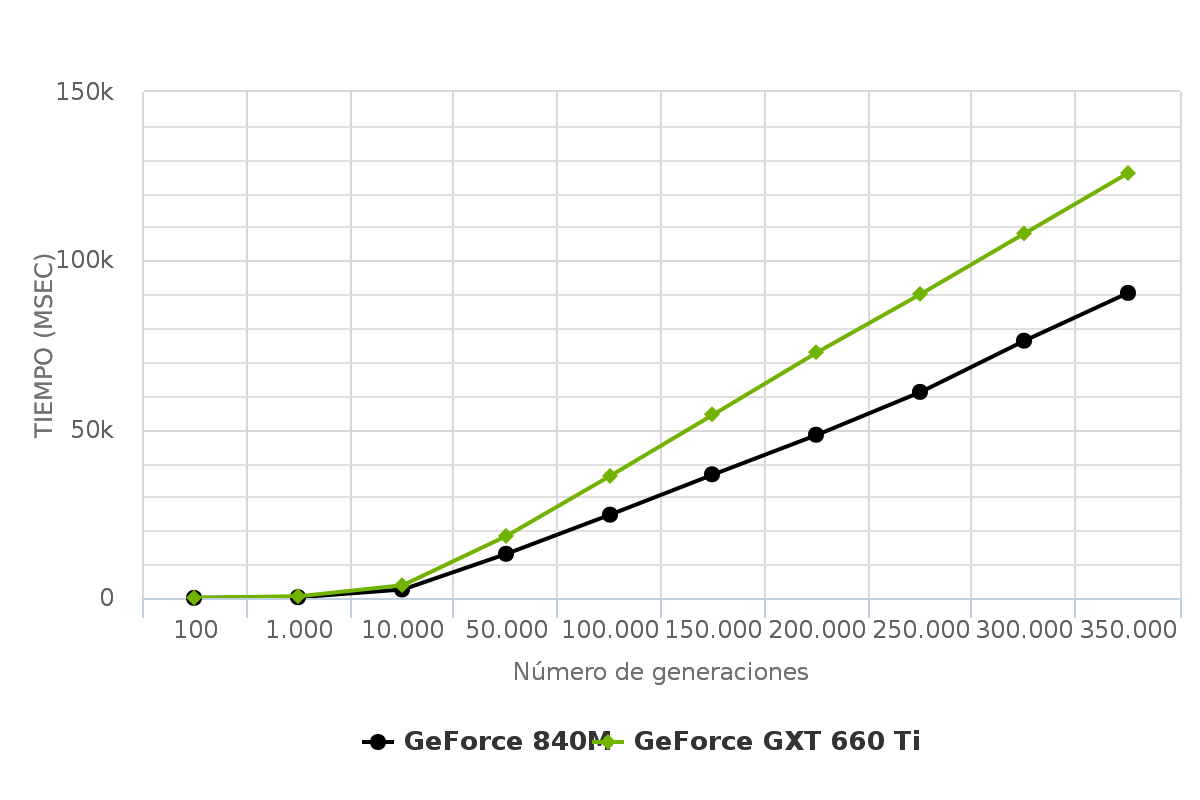
\includegraphics[width=0.9\linewidth]{../images/grafico_tiempos}
	\caption[Comparativa de tiempos entre tarjetas]{Comparativa de tiempos entre tarjetas}
	\label{fig:grafico_tiempos}
\end{figure}

\bigskip
Y se ve que la tarjeta con mejores prestaciones pero peor capacidad (GeForce GTX 660 Ti) tarda más en ejecutar los mismos procesamientos que hace la tarjeta con peores prestaciones pero mejor capacidad (GeForce 840M).

\bigskip
Como conclusión se llega a que a la hora de escoger el dispositivo a usar por el sistema para realizar los cómputos no sólo habrá que tener en cuenta los requisitos, si no que el factor de capacidad será decisivo para el rendimiento del cómputo y con ello del sistema.

También que ambas producen buenos resultados en el sistema, por lo que, se podría usar cualquiera en el sistema.


\chapter{Manuales}


\section{Manual de usuario}
\bigskip



\section{Manual de despliegue}
\bigskip

A continuación se explicará la forma y requisitos de despliegue del sistema. 

\subsection{Requisitos para el despliegue}
\bigskip

Para el correcto despliegue de la aplicación habrá que contar con sus 2 partes: el servicio web y el procesamiento con GPU mediante CUDA.

\bigskip
Para lanzar el servicio web:
\begin{itemize}
	\item Apache (versión 2.4 o superior)
	\item Python (Python 2)
	\item Django  (versión 1.10 o superior)
\end{itemize} 

\bigskip
Y para el procesamiento mediante CUDA:
\begin{itemize}
	\item Dispositivo NVIDIA
	\item Drivers NVIDIA (versión 352.xx)
	\item CUDA 7.5
	\item C++ (versión 4.x)
\end{itemize} 

\subsection{Despliegue}
\bigskip


Una vez que se cumplen los requisitos, sólo habrá que lanzar el servicio web, ya que el procesamiento usando la GPU se gestiona sólo mediante el ejecutable \textit{geneticAlgorithm}.

Para ello el servidor Apache tendrá que estar activo (se puede activar ejecutando \textit{service apache2 restart}) y lanzar el proyecto Django con el proyecto: dentro del directorio SWGPU ejecutar, junto con la URL donde lanzar el sistema \textit{python manage.py runserver [URL]}


\subsection{Despliegue automatizado}
\bigskip
También se proporcionará el script o archivo \textit{despliegue.sh} para automatizar la tarea de despliegue.

Simplemente habrá que ejecutarlo (dentro del \textit{directorio SWGPU},mediante la orden \textbf{sudo ./despliegue.sh}) y luego especificar la URL donde se desplegará. El script comprobará los requisitos antes citados, preparará el servidor y lanzará el sistema.

En la siguiente captura se ve como se lanza el servidor:

\bigskip
\begin{figure}[h]
	\centering
	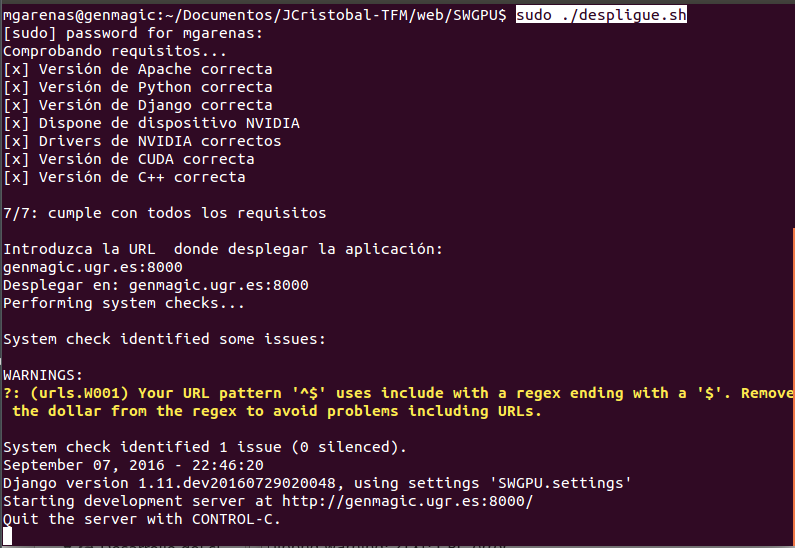
\includegraphics[width=1\linewidth]{../images/prueba_despliegue}
	\caption[Captura del despliegue automático]{Captura del despliegue automático}
	\label{fig:prueba_despliegue}
\end{figure}



\chapter{Conclusiones y trabajos futuros}


\bigskip
\section{Conclusiones}
\bigskip

Una vez realizado el trabajo, se verán los objetivos (citados en el capítulo 2) y su respectivo avance.

\bigskip
Respecto a las clases para lanzar un algoritmo genético se han logrado cumplir, reuniéndolas en el archivo ejecutable \textit{geneticAlgorithm}. Se ha desarrollado como un módulo independiente, para poder ser usado por cualquier servicio, y no ser dependiente del servicio web, controlando la entrada de parámetros y control de fallos.

\bigskip
También se ha creado la estructura del servicio web, de manera que sea accesible desde cualquier servidor web.
Dicho servicio facilita la petición del algoritmo genético, y se obtendrán los resultados mediante el uso de la GPU del servidor.

\bigskip
Se a publicado el servicio, en forma de \textit{beta}. Se encuentra accesible en  \href{www.genmagic.ugr.es:8000}{www.genmagic.ugr.es:8000}, accesible dentro de la red de la UGR \cite{vpnugr}.
	

\section{Trabajos futuros}

\bigskip
Además de mantener y gestionar la versión actual del servicio web, se podría trabajar en la mejora de la experiencia de usuario.

\bigskip
También se refinará el algoritmo, logrando un mejor aprovechamiento de los recursos y mejorando los resultados.

\bigskip
Como se comenta en el capítulo 6 (en la subsección \textit{Ejecutable a usar por el BackEnd}) se estudiará la posibilidad de que el usuario pudiera añadir funcionalidades o cualquier procesamiento usando la GPU mediante CUDA. 

\bigskip
De esta manera se podría ejecutar cualquier opción de optimización, o fuera del ámbito de los algoritmos genéticos cualquier funcionalidad que requiera el usuario.

\bigskip
Esto requeriría un conocimiento mayor por parte del usuario. Además supondría un mayor consumo de recursos, pero con un buen uso del usuario y una correcta prevención de fallos se conseguiría una funcionalidad mayor y llena de posibilidades. 











\newpage
%\bibliography{BIBLIO}
%\bibliographystyle{apalike}
\bibliography{bibliografia}\addcontentsline{toc}{chapter}{Bibliografía}
%\bibliographystyle{miunsrturl}
\bibliographystyle{ieeetr}


\end{document}
